%%%%%%%%%%%%%%%%%%%%%%%%%%%%%%%%%%%%%%%%%%%%%%%%%%%%%%%%%%%%%%%%%%%%%%
% LaTeX Template: Beamer arrows
%
% Source: http://www.texample.net/
% Feel free to distribute this template, but please keep the
% referal to TeXample.net.
% Date: Nov 2006
% 
%%%%%%%%%%%%%%%%%%%%%%%%%%%%%%%%%%%%%%%%%%%%%%%%%%%%%%%%%%%%%%%%%%%%%%
% How to use writeLaTeX: 
%
% You edit the source code here on the left, and the preview on the
% right shows you the result within a few seconds.
%
% Bookmark this page and share the URL with your co-authors. They can
% edit at the same time!
%
% You can upload figures, bibliographies, custom classes and
% styles using the files menu.
%
% If you're new to LaTeX, the wikibook is a great place to start:
% http://en.wikibooks.org/wiki/LaTeX
%
%%%%%%%%%%%%%%%%%%%%%%%%%%%%%%%%%%%%%%%%%%%%%%%%%%%%%%%%%%%%%%%%%%%%%%
% \documentclass[xcolor=dvipsnames,handout]{beamer} %
\documentclass[xcolor=dvipsnames]{beamer} %
\definecolor{purple}{rgb}{0.3098039 0.0000000 0.7411765}
\usetheme{Madrid}
\useoutertheme{miniframes} % Alternatively: miniframes, infolines, split
\useinnertheme{circles}
% \usecolortheme[named=UBCblue]{structure}
\setbeamercolor{palette primary}{bg=purple,fg=white}
\setbeamercolor{palette secondary}{bg=white,fg=white}
\setbeamercolor{palette tertiary}{bg=white,fg=white}

% \usepackage{hyperref} %allow for hyper links
% \hypersetup{bookmarks=false,colorlinks,%
% citecolor=blue,%
% filecolor=blue,%
% linkcolor=blue,%
% urlcolor=blue,%
% pdftex}
\usepackage[latin1]{inputenc}
\usefonttheme{professionalfonts}
\usepackage{times}
\usepackage{tikz}
\usepackage{amsmath,amssymb}
\usepackage{verbatim}
\usetikzlibrary{arrows,shapes}
\usepackage{cleveref}
\usepackage{lcg,calc}
\usepackage{multimedia}
% \newcommand{\pdfmovie}[4]{\href{run:#1}{\framebox{\parbox[c][#3][c]{#2}{\center #4}}}}
\usepackage{media9}

\author{Deshawn Sambrano}
\title{The Cost of Accumulating Evidence}

\begin{document}

\begin{comment}
:Title: Beamer arrows
:Tags: Remember picture, Beamer, Physics & chemistry, Overlays
:Use page: 3


To include videos you must run in adobe reader or acrobat.

With PGF/TikZ version 1.09 and later, it is possible to draw paths between nodes across
different pictures. This is a useful feature for presentations with the
Beamer package. In this example I've combined the new PGF/TikZ's overlay feature
with Beamer overlays. Download the PDF version to see the result.

**Note.** This only works with PDFTeX, and you have to run PDFTeX twice.

| Author: Deshawn Sambrano

\end{comment}
\begin{frame}[noframenumbering,plain]
  \titlepage
\end{frame}
% Need to add the subtitle with thier info, the citation thing






\begin{frame}{movie}
  \frametitle{Introduction to the Task}
  \begin{figure}[h!]
  \centering    
  \movie[width=1.0\textwidth, height=6.5cm,duration=1.5s] 
    {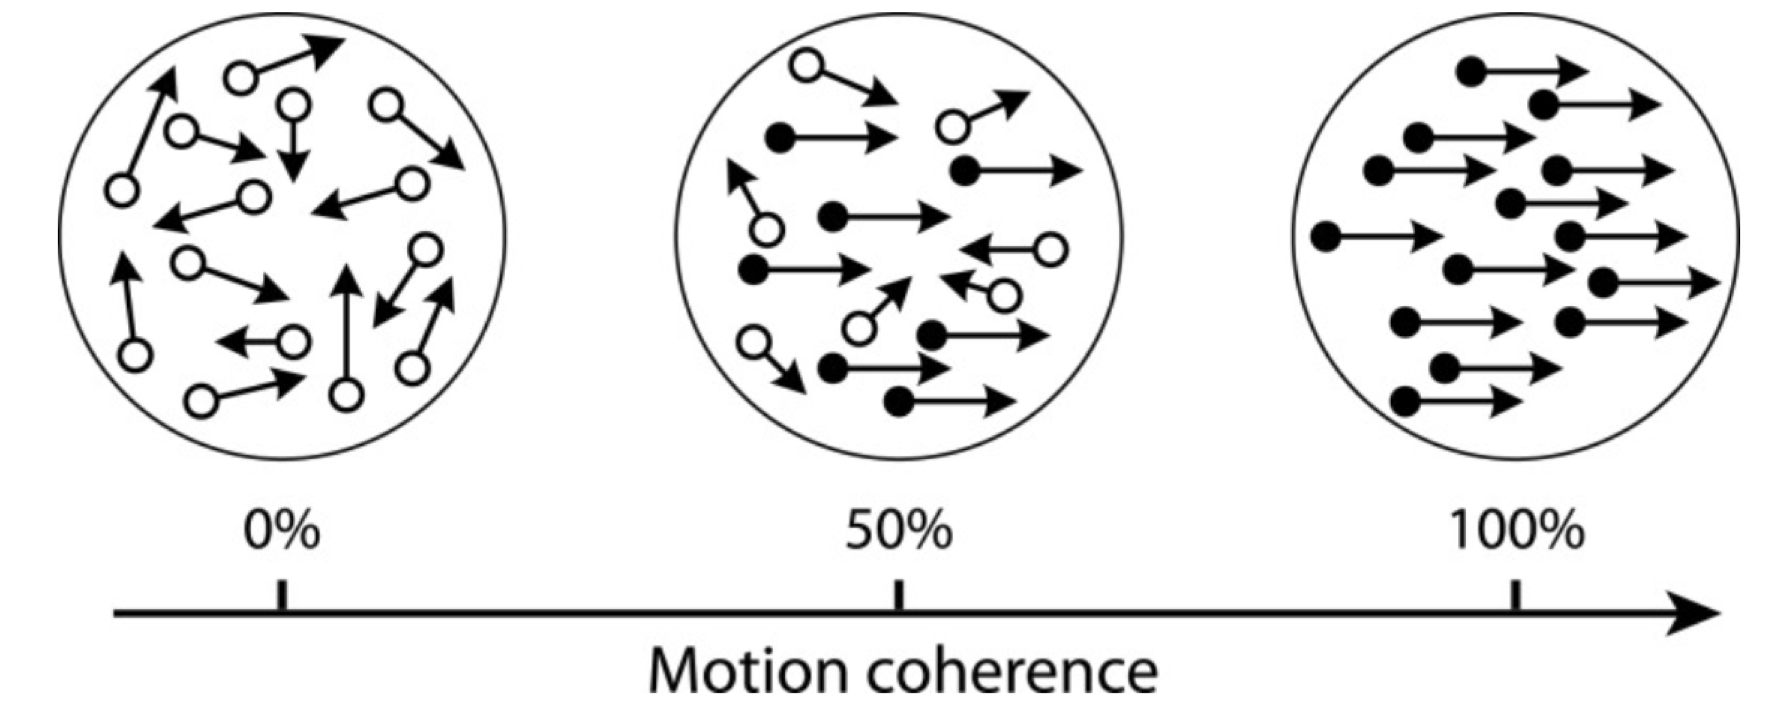
\includegraphics[width=1.0\textwidth]{RDMtask.png}}
	{Left_30.mov}
    % \caption{caption}
   \end{figure}
  % \centering \movie[open,showcontrols,width=9cm,height=5.25cm,poster]{\centering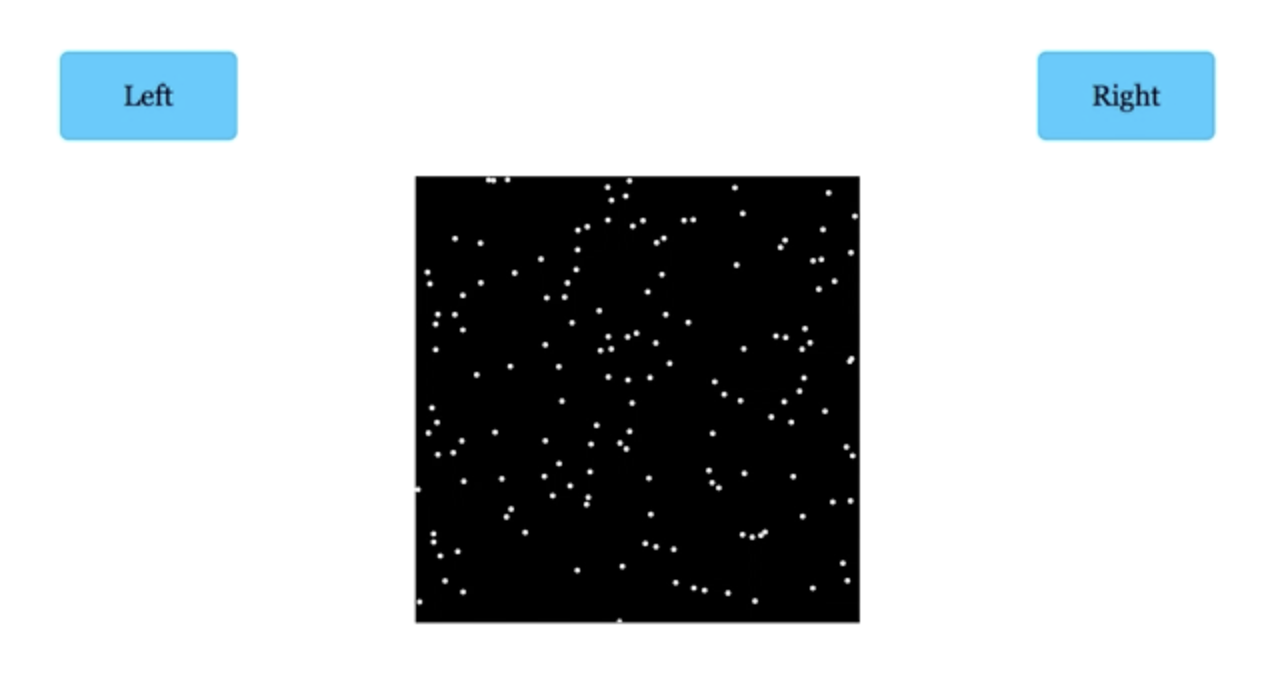
\includegraphics[width=6cm,height=3.5cm]{Left_30.png}}{Left_30.mov}
\end{frame}








\begin{frame}
  \frametitle{Drift Diffusion Model}
  \begin{figure}[h!]
	  \centering
  	 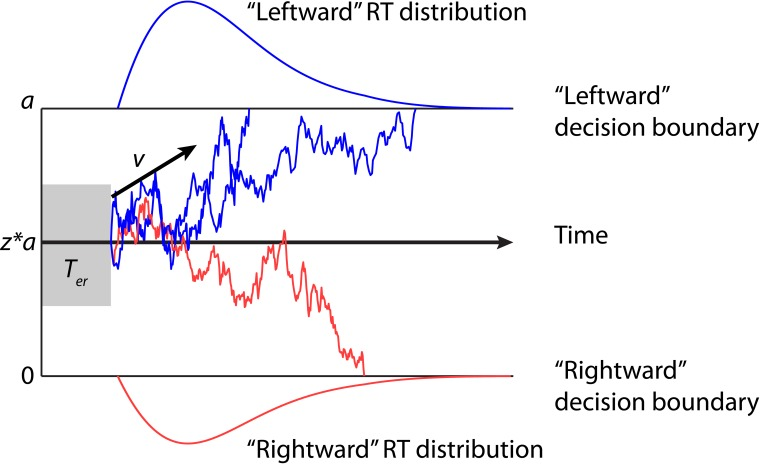
\includegraphics[width=.8\textwidth]{constantCostDDM.jpg}
  \end{figure}
\end{frame}










% By default all math in TikZ nodes are set in inline mode. Change this to
% displaystyle so that we don't get small fractions.
\everymath{\displaystyle}

\begin{frame}
	\frametitle{Step 1: Generative Model}
	\begin{figure}
		\begin{center}
			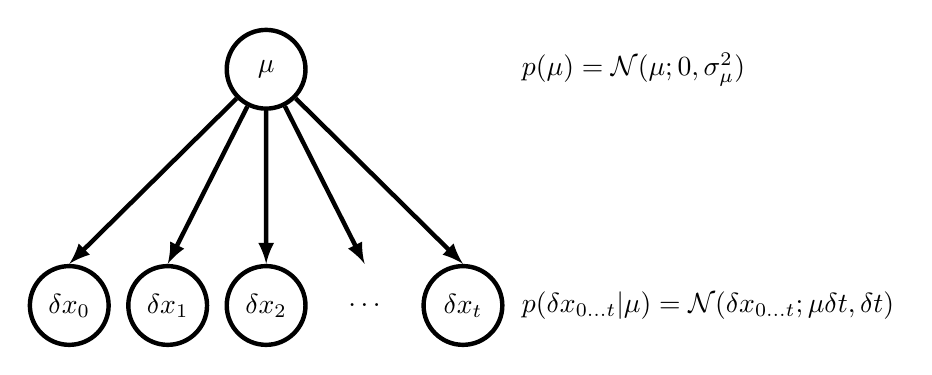
\begin{tikzpicture}[xscale=1.25]
				\tikzstyle{arrow}=[draw, -latex]
				\newcommand\Xmax{5}
				\newcommand\XMid{\Xmax/2}
				\newcommand\Xtext{\Xmax}

				\newcommand\YSpace{3}
				\newcommand\Yclass{1.5}
				\newcommand\YStim{\Yclass-\YSpace}
				\newcommand\Yxs{\YStim-\YSpace}

				% Grid
				% \draw [help lines] (0,-5) grid (7,3);
				 % Class
				% \node [draw, circle, minimum width=1cm, ultra thick] at (\XMid,\Yclass) (C) {$C$};
				% \node [anchor=west] at (\Xtext, \Yclass) (Cstat) {$p(C = 1) = .5$};

				 % Stimulus
				\node [draw, circle, minimum width=1cm, ultra thick] at (\XMid,\YStim) (mu) {$\mu$};
				\node [anchor=west, align=left] at (\Xtext, \YStim) (Cstat) {$p(\mu) = \mathcal{N}(\mu;0,\sigma_{\mu}^2)$};

				 % Observations
				\node [draw, circle, minimum width=1cm, ultra thick] at (.5,\Yxs) (x0) {$\delta x_0$};
				\node [draw, circle, minimum width=1cm, ultra thick] at (1.5,\Yxs) (x1) {$\delta x_1$};
				\node [draw, circle, minimum width=1cm, ultra thick] at (2.5,\Yxs) (x2) {$\delta x_2$};
				\node [draw, circle, minimum width=1cm, ultra thick, white] at (3.5,\Yxs) (dots) {\textcolor{black}{$\ldots$}};
				\node [draw, circle, minimum width=1cm, ultra thick] at (4.5,\Yxs) (xt) {$\delta x_t$};
				\node [anchor=west] at (\Xtext, \Yxs) (Cstat) {$p(\delta x_{0\hdots t}|\mu) = \mathcal{N}(\delta x_{0\hdots t};\mu\delta t,\delta t)$};
  
				 % Path Arrows 
				% \path [arrow, ultra thick] (C) -- (S);
 
				\path [arrow, ultra thick] (mu) -- (x0.north);
				\path [arrow, ultra thick] (mu) -- (x1.north);
				\path [arrow, ultra thick] (mu) -- (x2.north);
				\path [arrow, ultra thick] (mu) -- (dots.north);
				\path [arrow, ultra thick] (mu) -- (xt.north);
 
			\end{tikzpicture}
		\end{center}
	% \caption{\label{fig:GModel}Generative Model.}
	\end{figure}
\end{frame}




\begin{frame}
	\frametitle{Inference of Interests}
	\begin{itemize}
		\item sign($\mu$)
		\begin{itemize}
			\item $T_t$: trial time
			\item $t_i$: intertrial time
			\item $t_p$: time penalty for incorrect answers
			\item $R_{ij}$: reward for choosing hypothesis i when true was j.
		\end{itemize}
		\item $c(t)$: Momentary cost function: $C(T_d) = \int_0^{T_d} c(t)dt$
	\begin{gather*}
		\rho = \frac{<R> - <C(T_d)>}{<T_t> + <t_i> + <t_p>}
	\end{gather*}
		\item $g(t)$: Momentary belief function: $p(H_1|\delta x_{0\ldots t}) = p(\mu \geq 0 | \delta x_{0\ldots t})$
	\end{itemize}
		
\end{frame}













\begin{frame} % Step 2: Inference and Decision Rule (fold)


% For every picture that defines or uses external nodes, you'll have to
% apply the 'remember picture' style. To avoid some typing, we'll apply
% the style to all pictures.
\tikzstyle{every picture}+=[remember picture]


\frametitle{Step 2: Inference and Decision Rule}

\tikzstyle{na} = [baseline=-.5ex]

\begin{itemize}[<alert@>]
    \item Posterior
        \tikz[na] \node[coordinate] (n1) {};
\end{itemize}


% Below we mix an ordinary equation with TikZ nodes. Note that we have to
% adjust the baseline of the nodes to get proper alignment with the rest of
% the equation.
\begin{equation*}
        \tikz[baseline]{
            \node[fill=blue!20,anchor=base] (t1)
            {$p(\mu|\delta x_{0\ldots t})$};
        } \propto
        \tikz[baseline]{
            \node[fill=red!20, ellipse,anchor=base] (t2)
            {$\mathcal{N}(\mu;0,\sigma_{\mu}^2)$};
        } \prod_n
        \tikz[baseline]{
            \node[fill=green!20,anchor=base] (t3)
            {$\mathcal{N}(\delta x_{n};\mu\delta t,\delta t)$};
        }
\end{equation*}

\begin{itemize}
    \item Prior
        \tikz[na]\node [coordinate] (n2) {};
    \item Likelihood
        \tikz[na]\node [coordinate] (n3) {};
\end{itemize}
\uncover<+->
{\begin{gather*}
	p(\mu|\delta x_{0\ldots t})  = \mathcal{N}\left(\mu; \frac{x(t)}{t + \sigma_\mu^{-2}},\frac{1}{t + \sigma_\mu^{-2}}\right)\\
	{\scriptstyle\text{\tiny where, } x(t) = \sum_n \delta x_{n}\text{\tiny, and } t = \sum_n \delta t}
\end{gather*}}


% Now it's time to draw some edges between the global nodes. Note that we
% have to apply the 'overlay' style.
\begin{tikzpicture}[overlay]
        \path[->] (n1) edge [bend left] (t1);
        \path[->] (n2) edge [bend right] (t2);
        \path[->] (n3) edge [out=0, in=-90] (t3);
\end{tikzpicture}
\end{frame}
% section Step 2: Inference and Decision Rule (end)










\begin{frame} % Decision Rule (fold)
	\frametitle{Decision Rule}
	\begin{itemize}
		\item The decision rule is more complex that normal because we must determine not only what choice the optimal decider would choose but also when they would choose that option.
		\begin{gather*}
			\tilde{V}(g,t) = max \left\{\begin{split}
				&gR_{11} + (1-g)R_{12} - (<t_i> + (1-g)\bar{t_p})\rho\text{,}\\
				&(1-g)R_{22} + gR_{21} - (<t_i> + g\bar{t_p})\rho\text{,}\\
				&<\tilde{V}(g(t+\delta t),t + \delta t)|g,t>_{g(t+\delta t)} - c(t)\delta t - \rho\delta t
			\end{split}\right\}
		\end{gather*}
		\textit{\tiny $^*$We will remove the extra degrees of freedom and identify the optimal $\rho$ by setting $\tilde{V}(\textstyle\frac{1}{2},0) = 0$.}
	\end{itemize}
\end{frame}
% section Decision Rule (end)





\begin{frame} % Model Predictions (fold)
	\frametitle{Model Predictions: Accuracy}
	\begin{itemize}
		\item This model makes the prediction that participants accuracy will be derived by there belief function at the time of the decision. Thus, if we use the true drift rate, we will be able to obtain optimal accuracy for a given stimulus strength. 
		\item If have symmetric time varying bounds $\theta(t)$, we can solve for optimal accuracy with the following.
	\end{itemize}
		\begin{gather*}
			\theta(t) = \sqrt{t + \sigma_\mu^{-2}}\Phi^{-1}(g_\theta(t))\\
			p(x = \theta(t)| x = \pm\theta(t),t,\mu = \mu_0) = g(t,\mu_0) = \frac{1}{1+e^{2\theta(t)\mu_0}}
		\end{gather*}
\end{frame}
% section Model Predictions (end)














\begin{frame} % Cost Function (fold)
	\frametitle{Cost Function}
	\begin{itemize}
		\item One quintessential addition to this model above the DDM, is that we have a time varying momentary cost function $c(t)$. This function is unique to the individual and can be solved with the following formula. 
	\end{itemize}
		\begin{gather*}
			c(t) = \frac{1}{\delta t}\left(\begin{split}
				&<\tilde{V}(g(t+\delta t),t + \delta t)|g,t>_{g(t+\delta t)} - \\
				&gR_{11} - (1-g)R_{12} - \\&(<t_i> + (1-g_\theta(t))<t_p> + \delta t)\rho
			\end{split}\right)
		\end{gather*}
\end{frame}
% section Cost Function (end)




\begin{frame}
	\frametitle{Cascading Solutions}
	\begin{figure}
		\begin{center}
			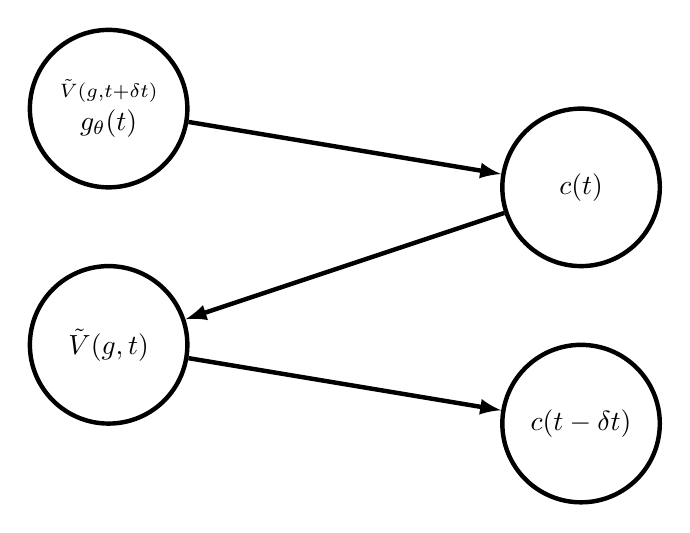
\begin{tikzpicture}[xscale=3]
				\tikzstyle{arrow}=[draw, -latex]
				\newcommand\XMax{1}
				\newcommand\XMin{-1}
				% \newcommand\Xtext{\Xmax}

				\newcommand\YSpace{3}
				\newcommand\Yclass{1.5}
				\newcommand\YTop{5}
				\newcommand\Yxs{\YStim-\YSpace}

				% Grid
				% \draw [help lines] (0,-5) grid (7,3);
				 % Class
				% \node [draw, circle, minimum width=1cm, ultra thick] at (\XMid,\Yclass) (C) {$C$};
				% \node [anchor=west] at (\Xtext, \Yclass) (Cstat) {$p(C = 1) = .5$};

				 % Stimulus
				\node [draw, circle, minimum width=2cm, ultra thick] at (\XMin,\YTop) (init) [draw, align=center]{$\scriptstyle\tilde{V}(g,t+\delta t)$\\$g_\theta(t)$};
				\node [draw, circle, minimum width=2cm, ultra thick] at (\XMax,\YTop-1) (ct) {$c(t)$};
				\node [draw, circle, minimum width=2cm, ultra thick] at (\XMin,\YTop-3) (Vt) [draw, align=center]{$\tilde{V}(g,t)$};
				\node [draw, circle, minimum width=2cm, ultra thick] at (\XMax,\YTop-3-1) (ct-1) {$c(t - \delta t)$};

				% Path Arrows
				\path [arrow, ultra thick] (init) -- (ct);
				
				\path [arrow, ultra thick] (ct) -- (Vt);
				\path [arrow, ultra thick] (Vt) -- (ct-1);
				% \path [arrow, ultra thick] (mu) -- (dots.north);
				% \path [arrow, ultra thick] (mu) -- (xt.north);
 
			\end{tikzpicture}
		\end{center}
	% \caption{\label{fig:GModel}Generative Model.}
	\end{figure}
\end{frame}








\begin{frame} % Changing Parameters (fold)
	\frametitle{Changing Parameters}
	\begin{figure}
	    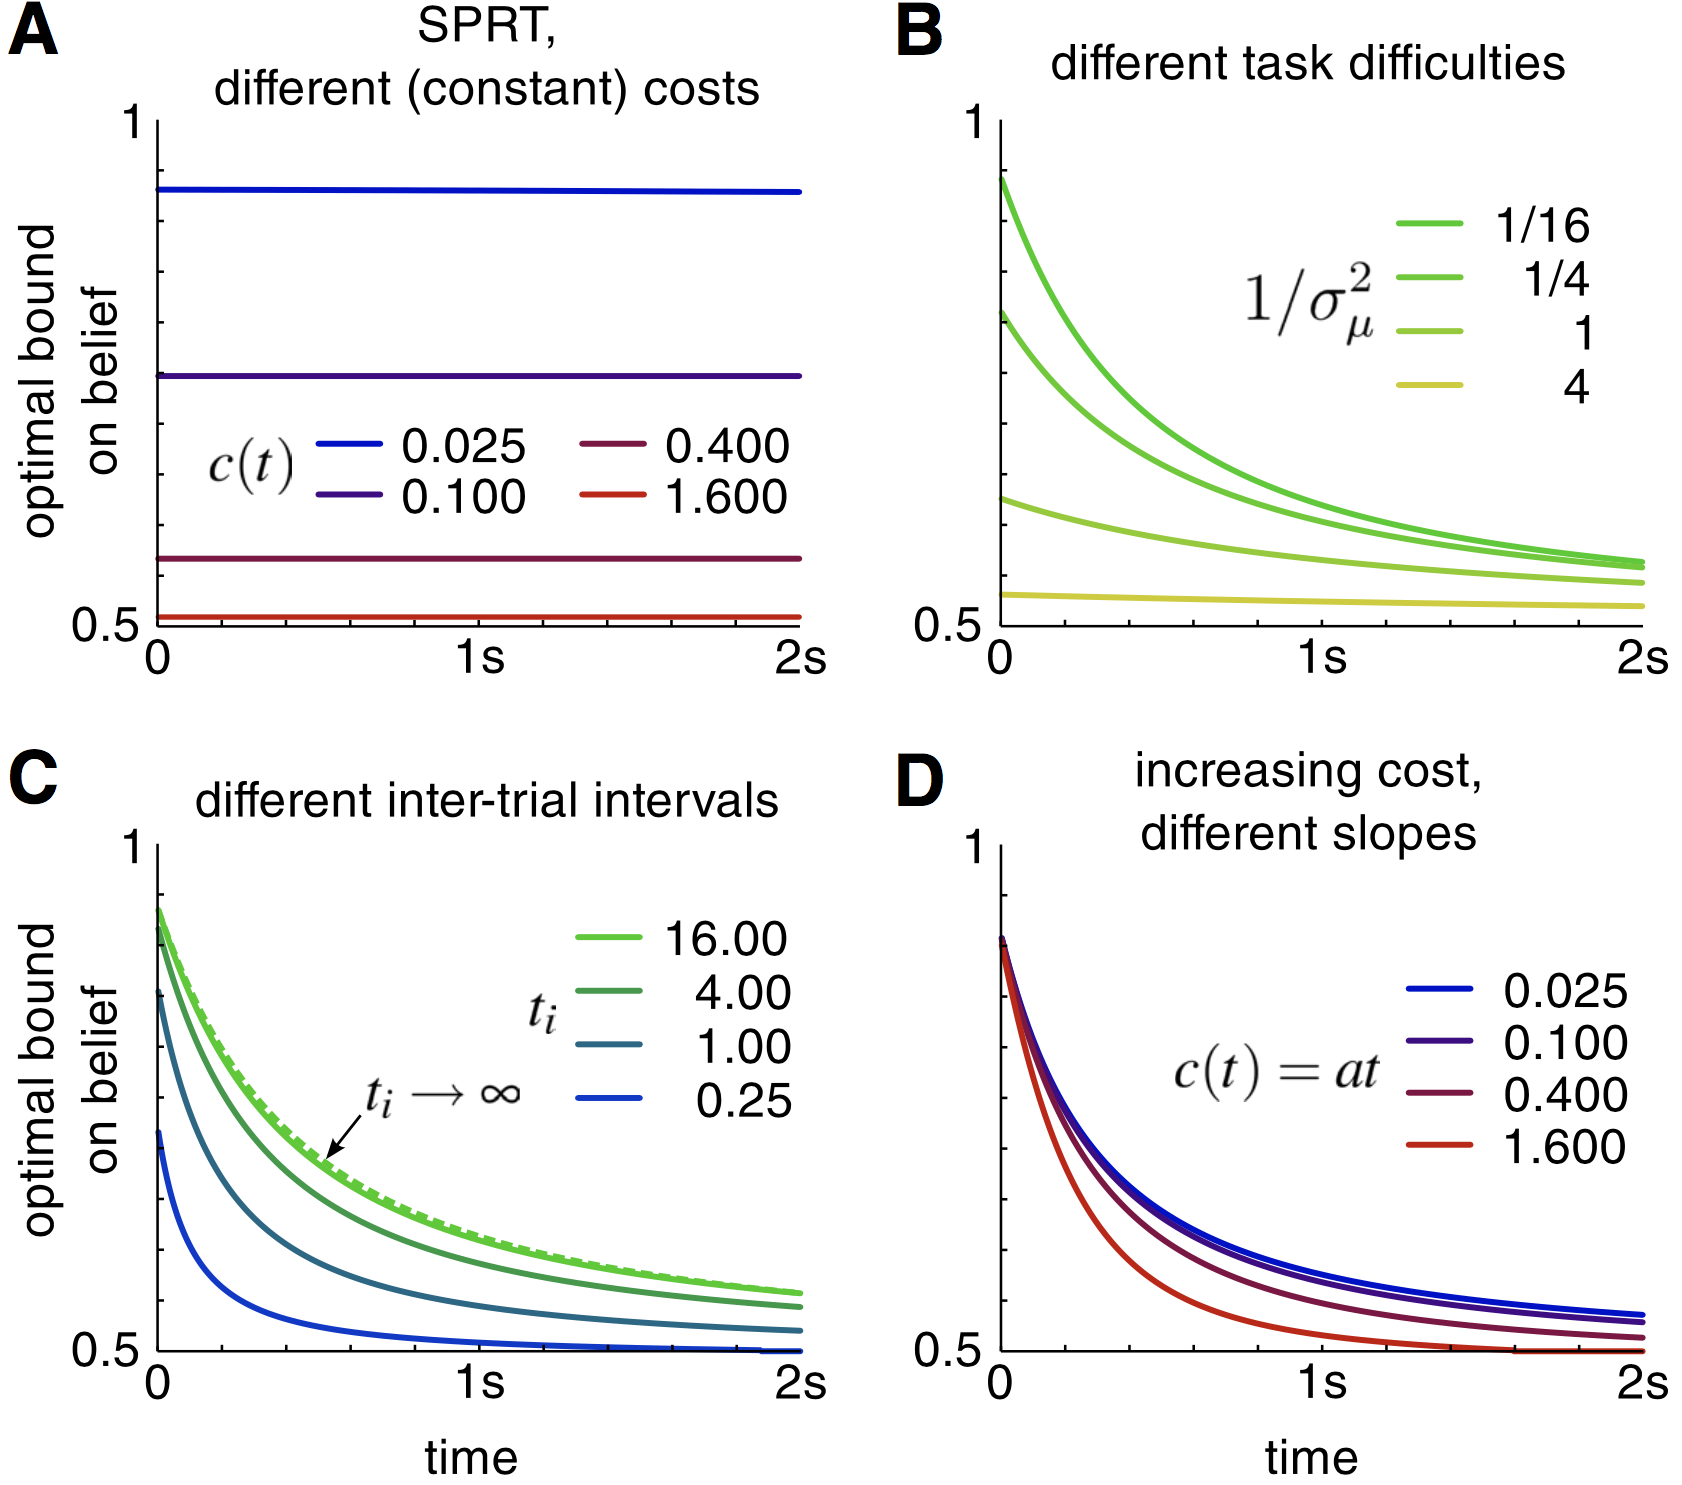
\includegraphics[height=.8\textheight]{Parameters.png}
	\end{figure}
\end{frame}
% section Changing Parameters (end)














\begin{frame}
  \frametitle{Dynamic decision boundaries}
    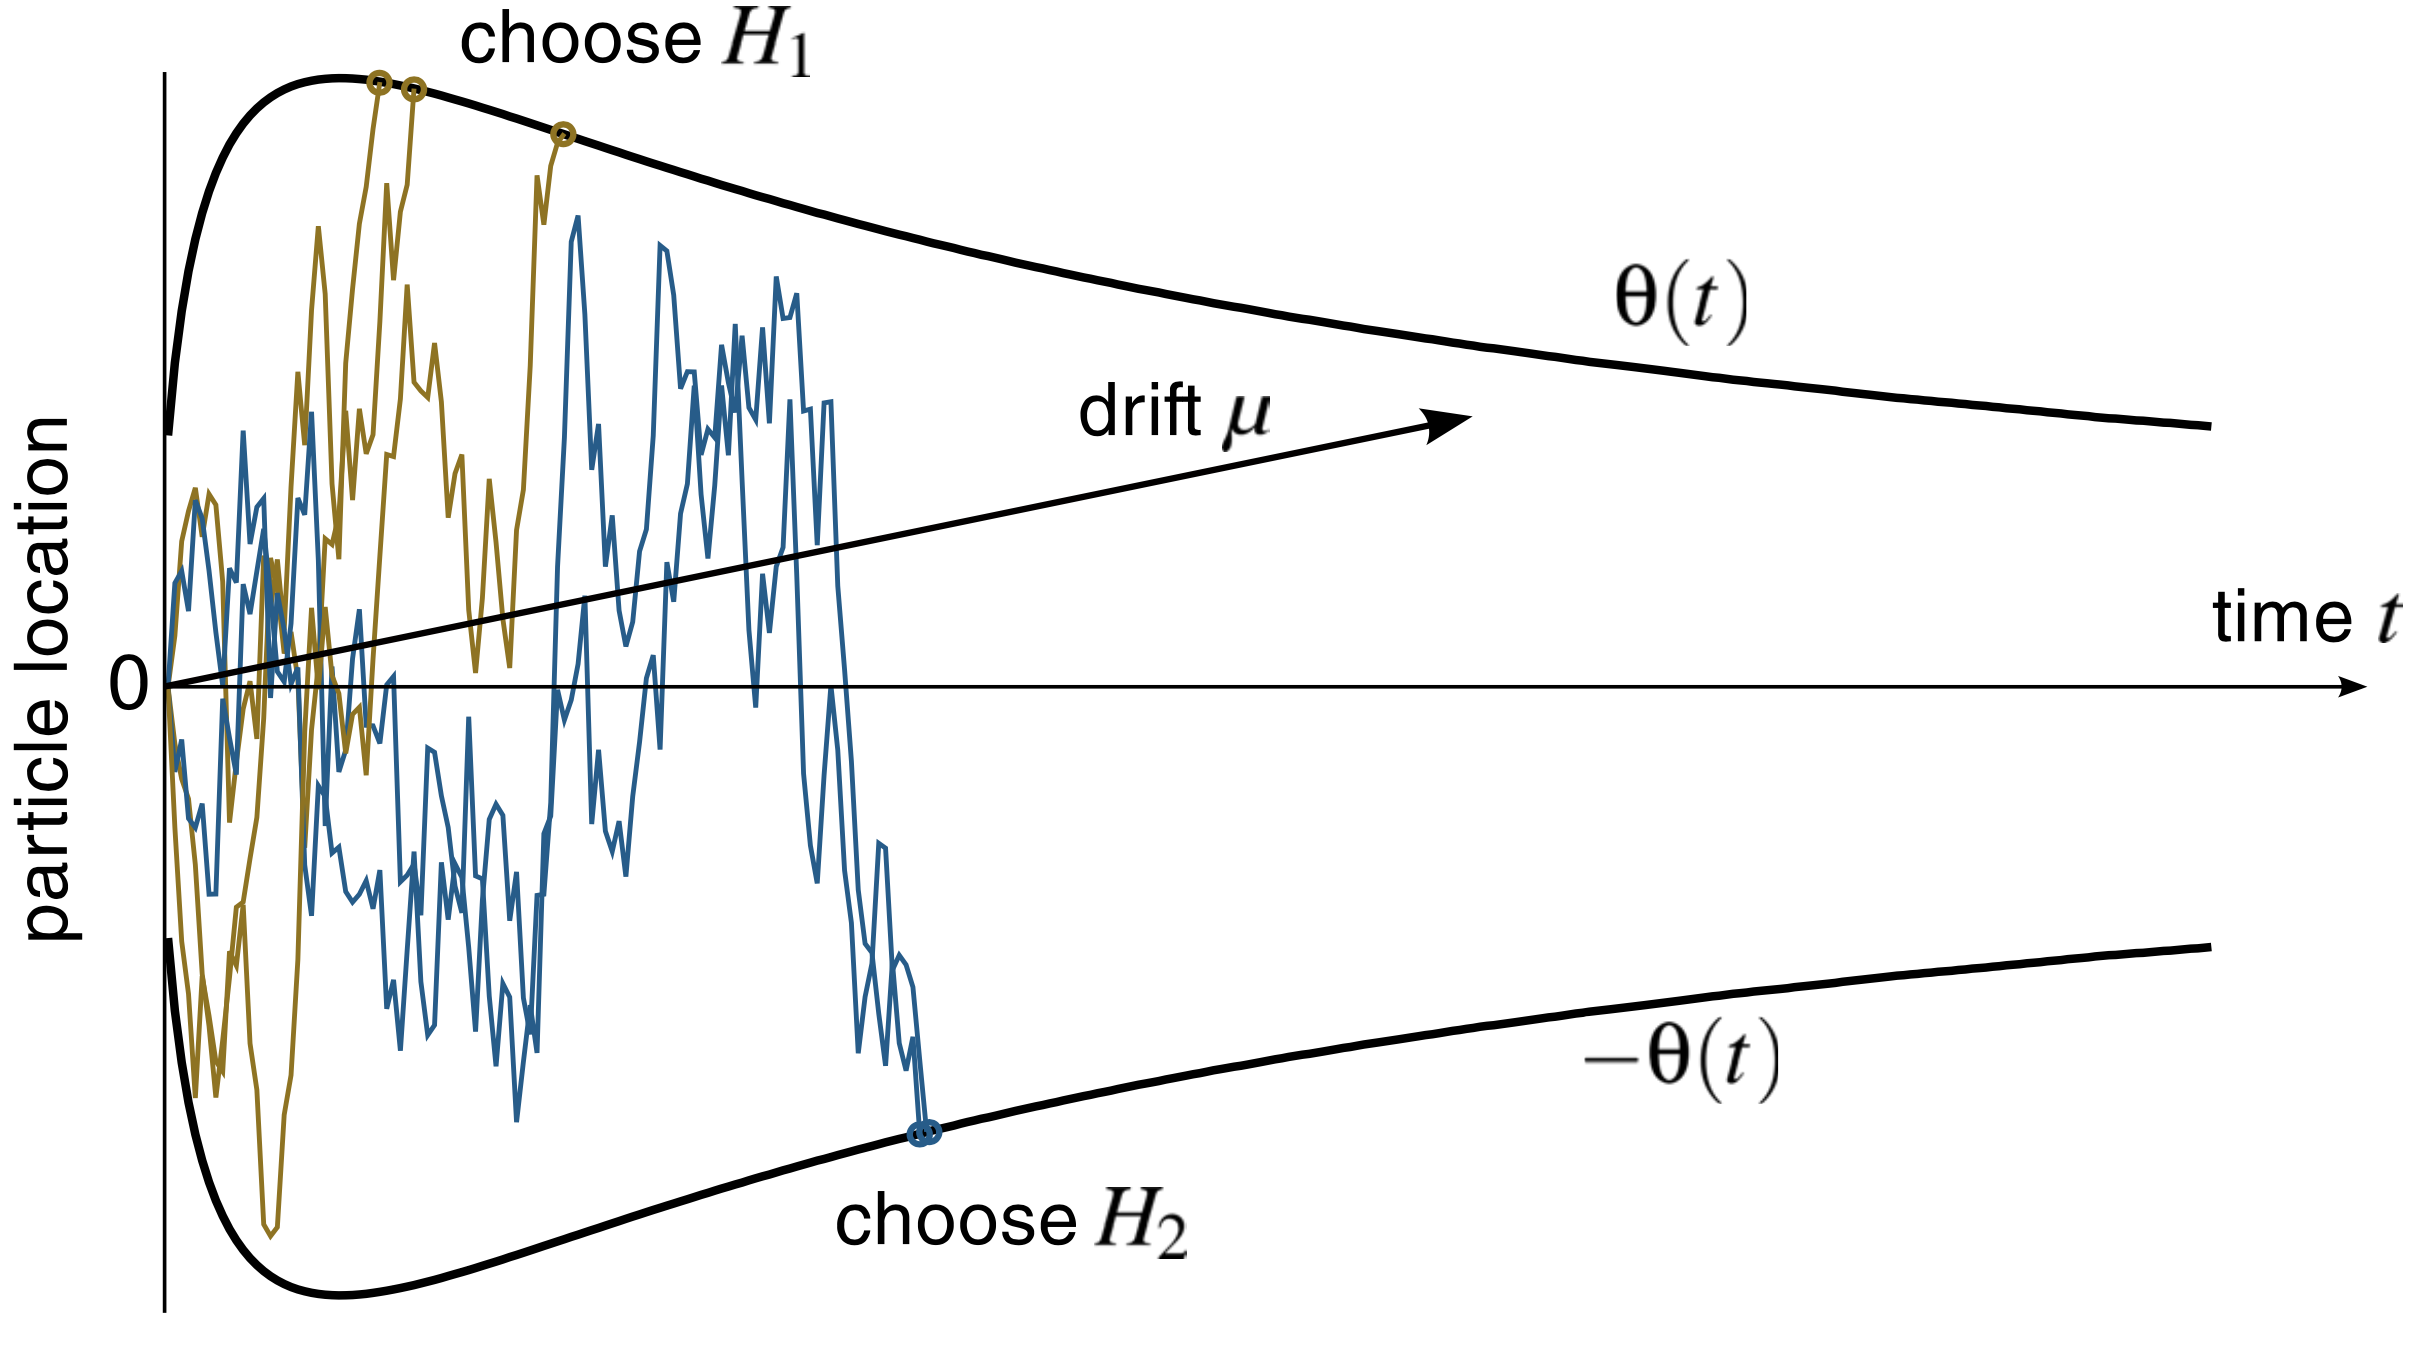
\includegraphics[width=\textwidth]{DDM.png}
\end{frame}

















\begin{frame} % Model Fit (fold)
	\frametitle{Model Fit}
    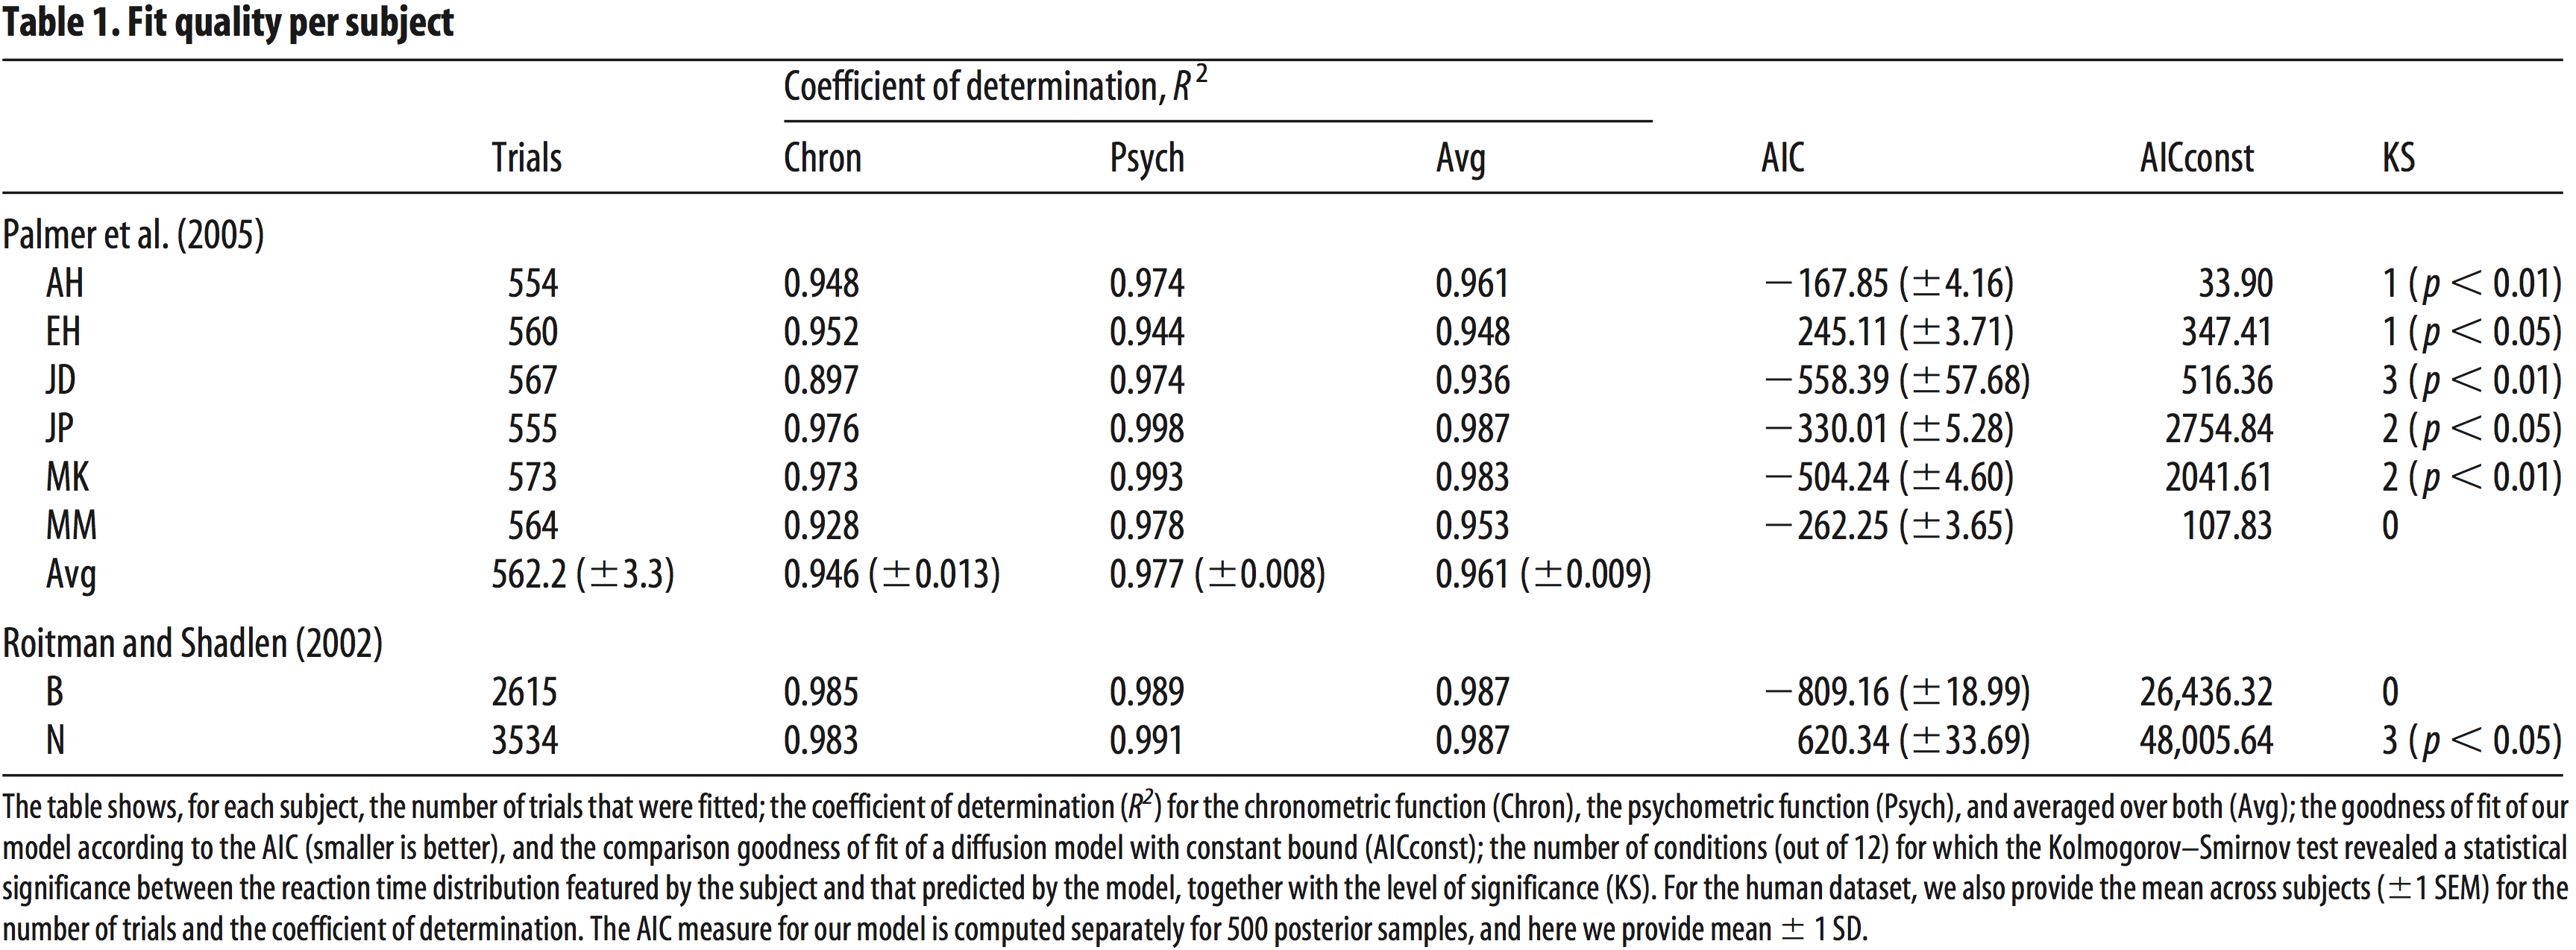
\includegraphics[width=\textwidth]{ModelFit.png}
\end{frame}
% section Model Fit (end)














\begin{frame} % Conclusion (fold)
	\frametitle{Conclusion}
\end{frame}
% section Conclusion (end)






\begin{frame} %  (fold)
\begin{figure}
	\centering
	
\begin{tikzpicture}
		\node at (0,0) (x) {\huge\color{purple}QUESTIONS?};
	\end{tikzpicture}
\end{figure}
\begin{itemize}
	\item For more information:
		\begin{itemize}
			\item \href{dsambrano.com}{\color{blue}\underline{DSambrano.com}}
			\item \href{mailto:dsambranonyu.edu}{\color{blue}\underline{DSambrano@nyu.edu}}
		\end{itemize}
\end{itemize}
\end{frame}
% section  (end)




















				% \node [draw, circle, minimum width=2cm, ultra thick] at (\XMin,\YTop) (init) [draw, align=center]{$\scriptstyle\tilde{V}(g,t+\delta t)$\\$g_\theta(t)$};




































% % For every picture that defines or uses external nodes, you'll have to
% % apply the 'remember picture' style. To avoid some typing, we'll apply
% % the style to all pictures.
% \tikzstyle{every picture}+=[remember picture]
%
%
% \begin{frame}
% \frametitle{Rigid body dynamics}
%
% \tikzstyle{na} = [baseline=-.5ex]
%
% \begin{itemize}[<+-| alert@+>]
%     \item Coriolis acceleration
%         \tikz[na] \node[coordinate] (n1) {};
% \end{itemize}
%
% % p(\mu|\delta x_{0\ldots t}) \propto \mathcal{N}(\mu;0,\sigma_{\mu}^2) \prod_n \mathcal{N}(\delta x_{n};\mu\delta t,\delta t)
%
% % Below we mix an ordinary equation with TikZ nodes. Note that we have to
% % adjust the baseline of the nodes to get proper alignment with the rest of
% % the equation.
% \begin{equation*}
% \vec{a}_p = \vec{a}_o+\frac{{}^bd^2}{dt^2}\vec{r} +
%         \tikz[baseline]{
%             \node[fill=blue!20,anchor=base] (t1)
%             {$ 2\vec{\omega}_{ib}\times\frac{{}^bd}{dt}\vec{r}$};
%         } +
%         \tikz[baseline]{
%             \node[fill=red!20, ellipse,anchor=base] (t2)
%             {$\vec{\alpha}_{ib}\times\vec{r}$};
%         } +
%         \tikz[baseline]{
%             \node[fill=green!20,anchor=base] (t3)
%             {$\vec{\omega}_{ib}\times(\vec{\omega}_{ib}\times\vec{r})$};
%         }
% \end{equation*}
%
% \begin{itemize}[<+-| alert@+>]
%     \item Transversal acceleration
%         \tikz[na]\node [coordinate] (n2) {};
%     \item Centripetal acceleration
%         \tikz[na]\node [coordinate] (n3) {};
% \end{itemize}
%
% % Now it's time to draw some edges between the global nodes. Note that we
% % have to apply the 'overlay' style.
% \begin{tikzpicture}[overlay]
%         \path[->]<1-> (n1) edge [bend left] (t1);
%         \path[->]<2-> (n2) edge [bend right] (t2);
%         \path[->]<3-> (n3) edge [out=0, in=-90] (t3);
% \end{tikzpicture}
% \end{frame}
\end{document}